% ======================= CHAPTER 4: EXPERIMENTS AND RESULTS ==========================
\chapter{Experiments and Results}

This chapter presents the experimental results of our study. We first compare the four individual models, then analyze the ensemble approach, followed by Grad-CAM visualizations and the ablation study.

All experiments were conducted on a single NVIDIA GPU using mixed-precision training (FP16) with PyTorch 2.x. The random seed was fixed at 42 for reproducibility.

\section{Individual Model Comparison}

\subsection{Overall Performance}

Table~\ref{tab:model_comparison} summarizes the test-set performance of all four architectures trained with the optimized pipeline.

\begin{table}[H]
\centering
\caption{Test-set performance comparison of the four evaluated architectures. Best values are highlighted in \textbf{bold}.}
\label{tab:model_comparison}
\begin{tabular}{lccccc}
\toprule
\textbf{Model} & \textbf{Accuracy} & \textbf{Macro F1} & \textbf{AUC} & \textbf{MCC} & \textbf{Kappa} \\
\midrule
EfficientNet-B0 & \textbf{0.8836} & \textbf{0.8311} & 0.9522 & \textbf{0.7721} & \textbf{0.7710} \\
ResNet50        & 0.8603 & 0.7902 & 0.9565 & 0.7310 & 0.7309 \\
DenseNet121     & 0.8543 & 0.7967 & 0.9587 & 0.7209 & 0.7206 \\
Swin-Tiny       & 0.8490 & 0.7855 & \textbf{0.9600} & 0.7157 & 0.7150 \\
\bottomrule
\end{tabular}
\end{table}

EfficientNet-B0 achieved the highest accuracy (88.36\%) and macro F1-score (0.831) among all individual models, despite being the smallest architecture with only 5.3M parameters. This result underscores the effectiveness of compound scaling~\cite{tan2019efficientnet}: EfficientNet achieves superior feature extraction with significantly fewer parameters than ResNet50 (25.6M) or Swin-Tiny (28M).\footnote{The relatively high test cross-entropy loss (0.75) observed for all models is an expected artifact of label smoothing training~\cite{muller2019does}: since the models are trained with soft targets ($\epsilon=0.1$), they learn to output maximum confidence $\approx 1 - \epsilon + \epsilon/C \approx 0.93$ rather than 1.0, resulting in higher raw loss values that do not reflect degraded classification quality.}

An intriguing pattern emerges when comparing accuracy against AUC. While EfficientNet-B0 leads in hard-classification metrics (accuracy, F1), Swin-Tiny achieves the highest AUC (0.960). This suggests that the self-attention mechanism of Transformers~\cite{dosovitskiy2021image} produces better-calibrated probability distributions, even though its discrete classification decisions are slightly less accurate on this relatively small dataset. This finding is consistent with the literature suggesting that Vision Transformers require larger datasets to fully exploit their modeling capacity~\cite{touvron2021deit}.

\subsection{Per-Class Analysis}

Table~\ref{tab:per_class_f1} presents the per-class F1-scores and AUC values for each model.

\begin{table}[H]
\centering
\caption{Per-class F1-scores and AUC values for each model on the test set.}
\label{tab:per_class_f1}
\begin{tabular}{l|cc|cc|cc|cc}
\toprule
\textbf{Class} & \multicolumn{2}{c|}{\textbf{EB0}} & \multicolumn{2}{c|}{\textbf{RN50}} & \multicolumn{2}{c|}{\textbf{DN121}} & \multicolumn{2}{c}{\textbf{Swin-T}} \\
 & F1 & AUC & F1 & AUC & F1 & AUC & F1 & AUC \\
\midrule
AKIEC & \textbf{0.717} & 0.921 & 0.646 & \textbf{0.949} & 0.637 & 0.928 & 0.660 & 0.949 \\
BCC   & \textbf{0.865} & \textbf{0.984} & 0.837 & 0.977 & 0.815 & 0.989 & 0.800 & 0.993 \\
BKL   & \textbf{0.758} & \textbf{0.938} & 0.730 & 0.926 & 0.741 & 0.945 & 0.698 & 0.947 \\
DF    & \textbf{0.938} & 0.963 & 0.800 & 0.981 & 0.867 & \textbf{0.992} & 0.914 & 0.942 \\
MEL   & \textbf{0.695} & 0.913 & 0.634 & 0.922 & 0.642 & 0.922 & 0.625 & \textbf{0.930} \\
NV    & \textbf{0.940} & 0.946 & 0.929 & 0.944 & 0.920 & 0.946 & 0.921 & \textbf{0.960} \\
VASC  & 0.905 & \textbf{1.000} & \textbf{0.955} & 0.997 & \textbf{0.955} & 0.989 & 0.880 & \textbf{1.000} \\
\bottomrule
\end{tabular}
\end{table}

Several important observations can be drawn from this per-class analysis:

\textbf{Melanoma (MEL)} remains the most challenging class across all models, with F1-scores ranging from 0.625 (Swin-Tiny) to 0.695 (EfficientNet-B0). This difficulty arises from melanoma's morphological overlap with benign keratosis (BKL) and melanocytic nevi (NV). However, melanoma AUC values range from 0.913 to 0.930, indicating that models can rank melanoma cases with reasonable confidence even when the hard classification threshold is suboptimal.

\textbf{Dermatofibroma (DF)} achieves remarkably high F1-scores (0.800--0.938) despite being the rarest class with only 17 test samples. This suggests that DF has distinctive visual features that are well-captured by transfer learning, and that the Weighted Random Sampler effectively compensates for its scarcity. However, these results should be interpreted with caution: with only 17 test samples, a single additional misclassification would reduce the F1-score by approximately 0.06, making these estimates sensitive to individual predictions.

\textbf{Vascular Lesion (VASC)} is consistently well-classified, with F1-scores between 0.880 and 0.955 and near-perfect AUC values (similarly based on a small test set of 22 samples). The distinctive red-purple coloration of vascular lesions provides strong discriminative signals for all architectures.

\subsection{Training Dynamics}

Figure~\ref{fig:training_history} shows the training and validation loss curves for all four models. All models demonstrate healthy convergence without significant overfitting, validating the effectiveness of the combined regularization strategy (Mixup + CutMix + Label Smoothing + Weight Decay).

\begin{figure}[H]
\centering
\begin{subfigure}{\textwidth}
    \makebox[\textwidth][c]{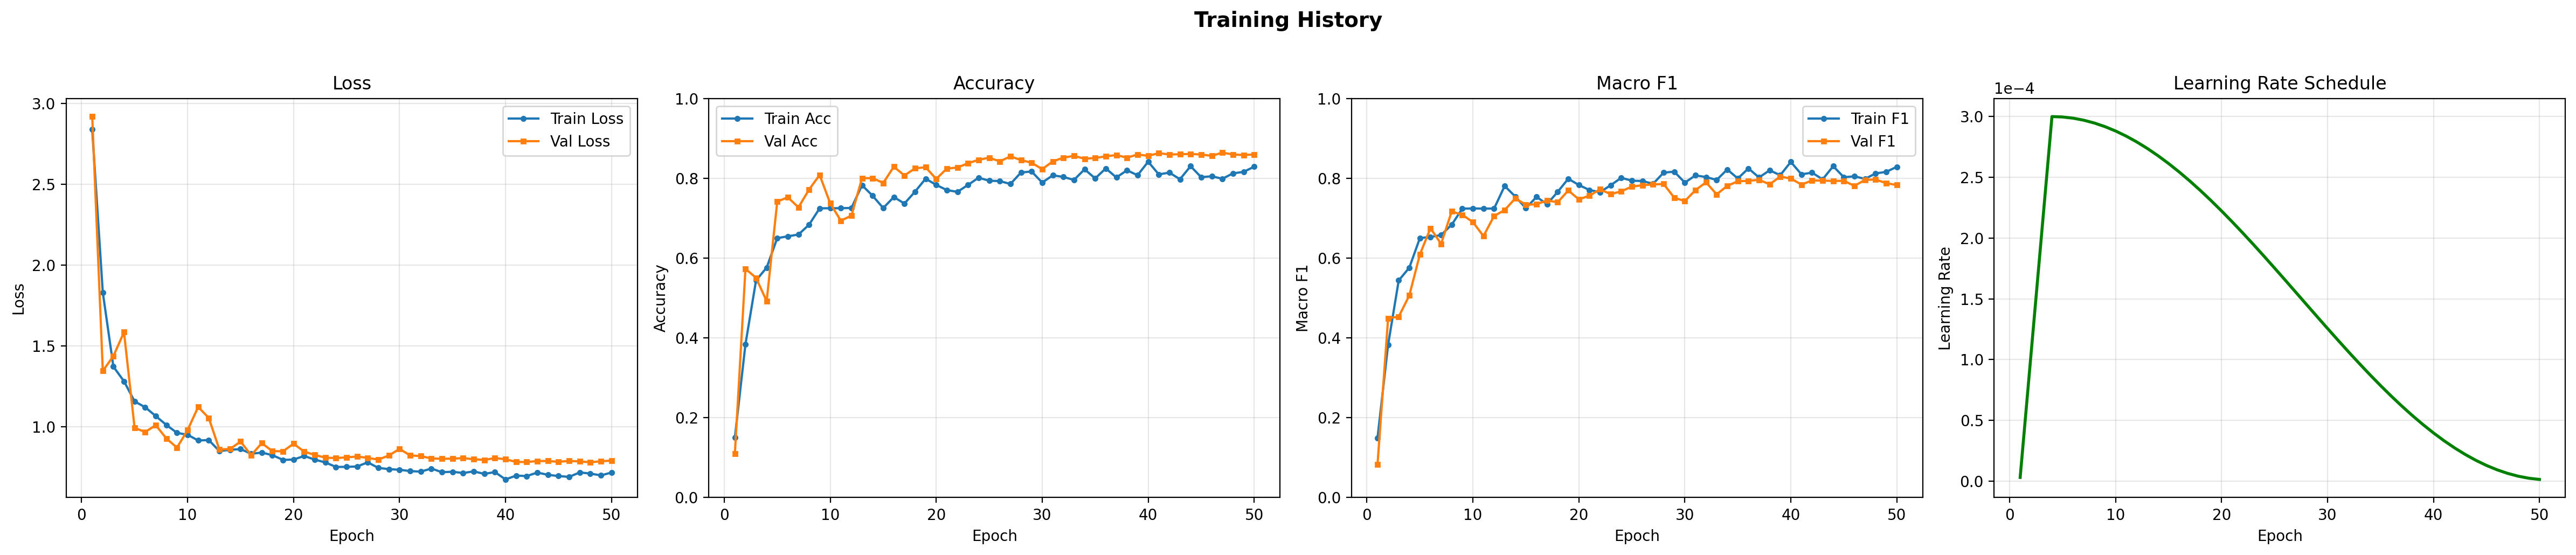
\includegraphics[width=1.15\textwidth]{figures/eb0_training_history.png}}
    \caption{EfficientNet-B0}
\end{subfigure}

\vspace{0.6cm}

\begin{subfigure}{\textwidth}
    \makebox[\textwidth][c]{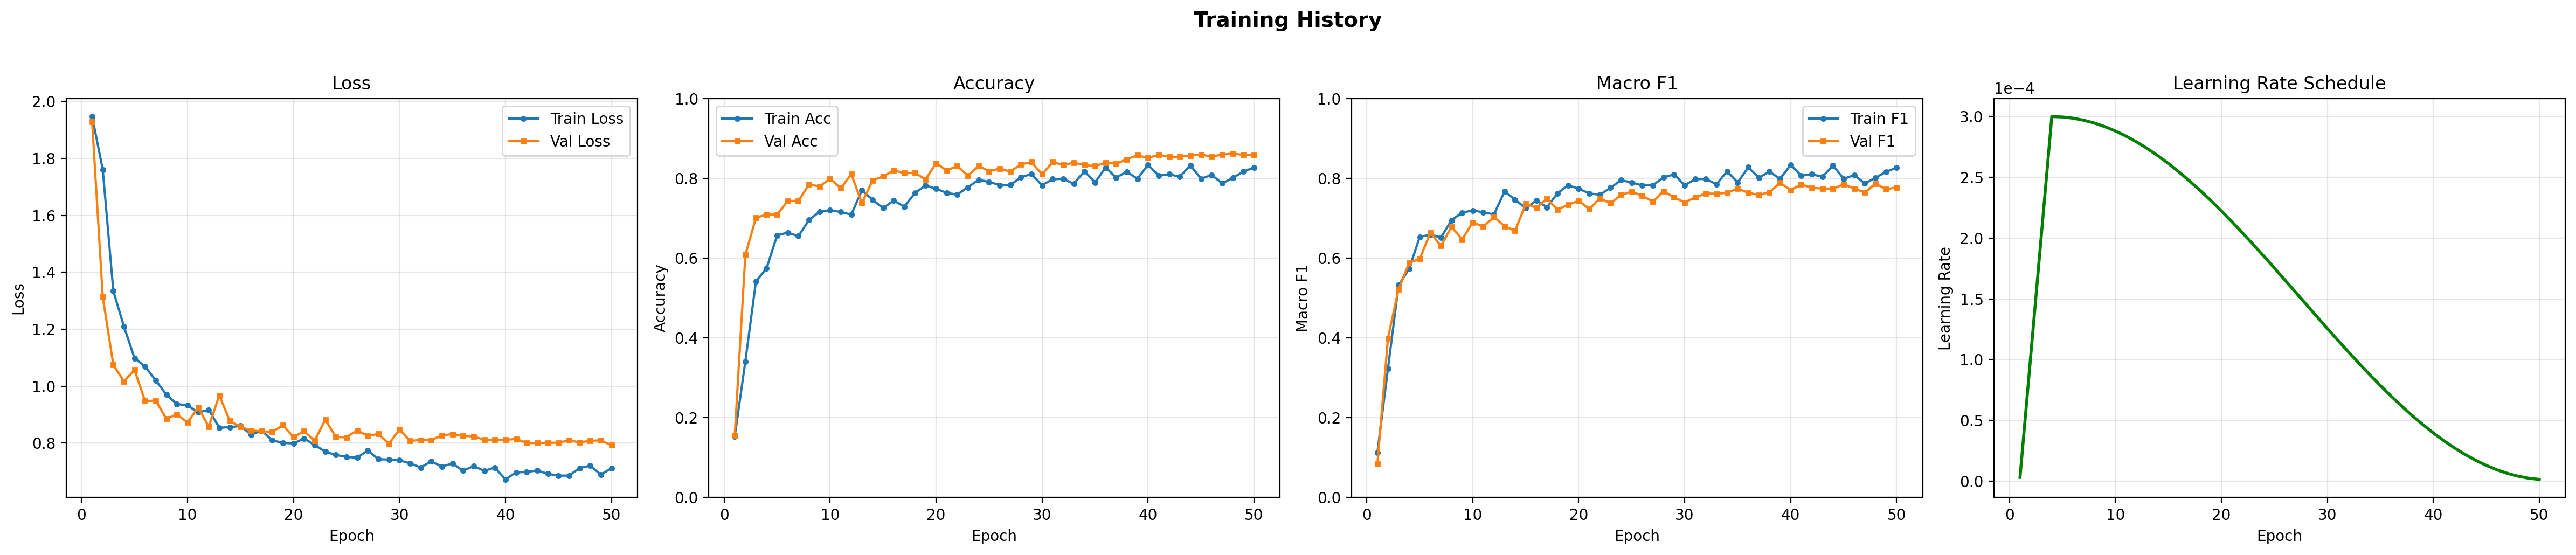
\includegraphics[width=1.15\textwidth]{figures/rn50_training_history.png}}
    \caption{ResNet50}
\end{subfigure}
\caption{Training history for all four models, showing loss, accuracy, and learning rate progression across epochs. All models demonstrate stable convergence without overfitting.}
\label{fig:training_history}
\end{figure}

\begin{figure}[H]
\ContinuedFloat
\centering
\begin{subfigure}{\textwidth}
    \makebox[\textwidth][c]{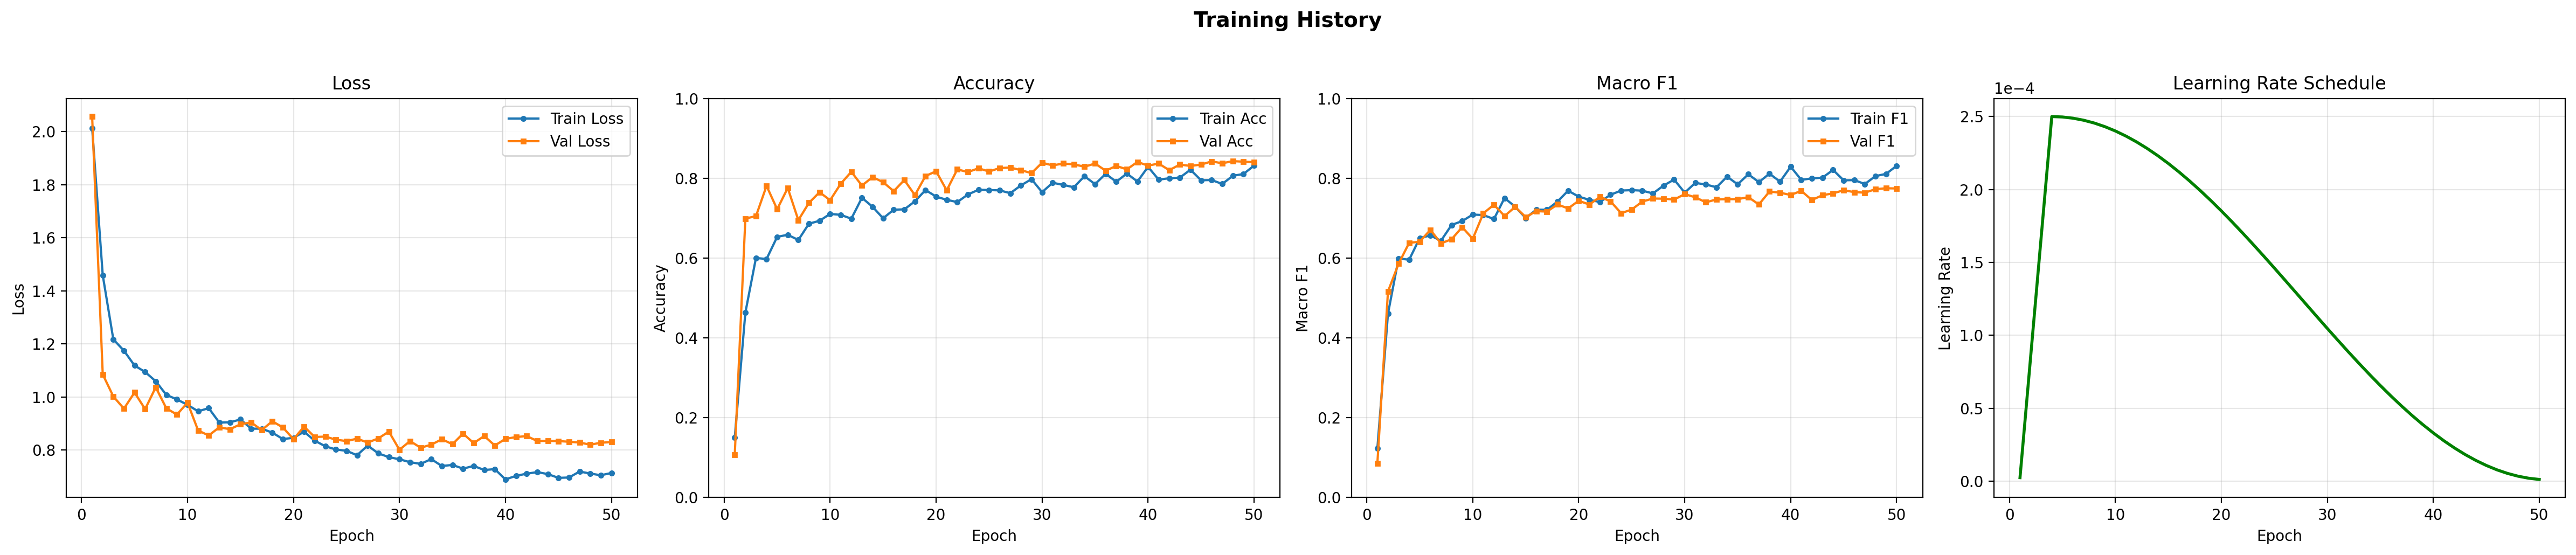
\includegraphics[width=1.15\textwidth]{figures/dn121_training_history.png}}
    \caption{DenseNet121}
\end{subfigure}

\vspace{0.6cm}

\begin{subfigure}{\textwidth}
    \makebox[\textwidth][c]{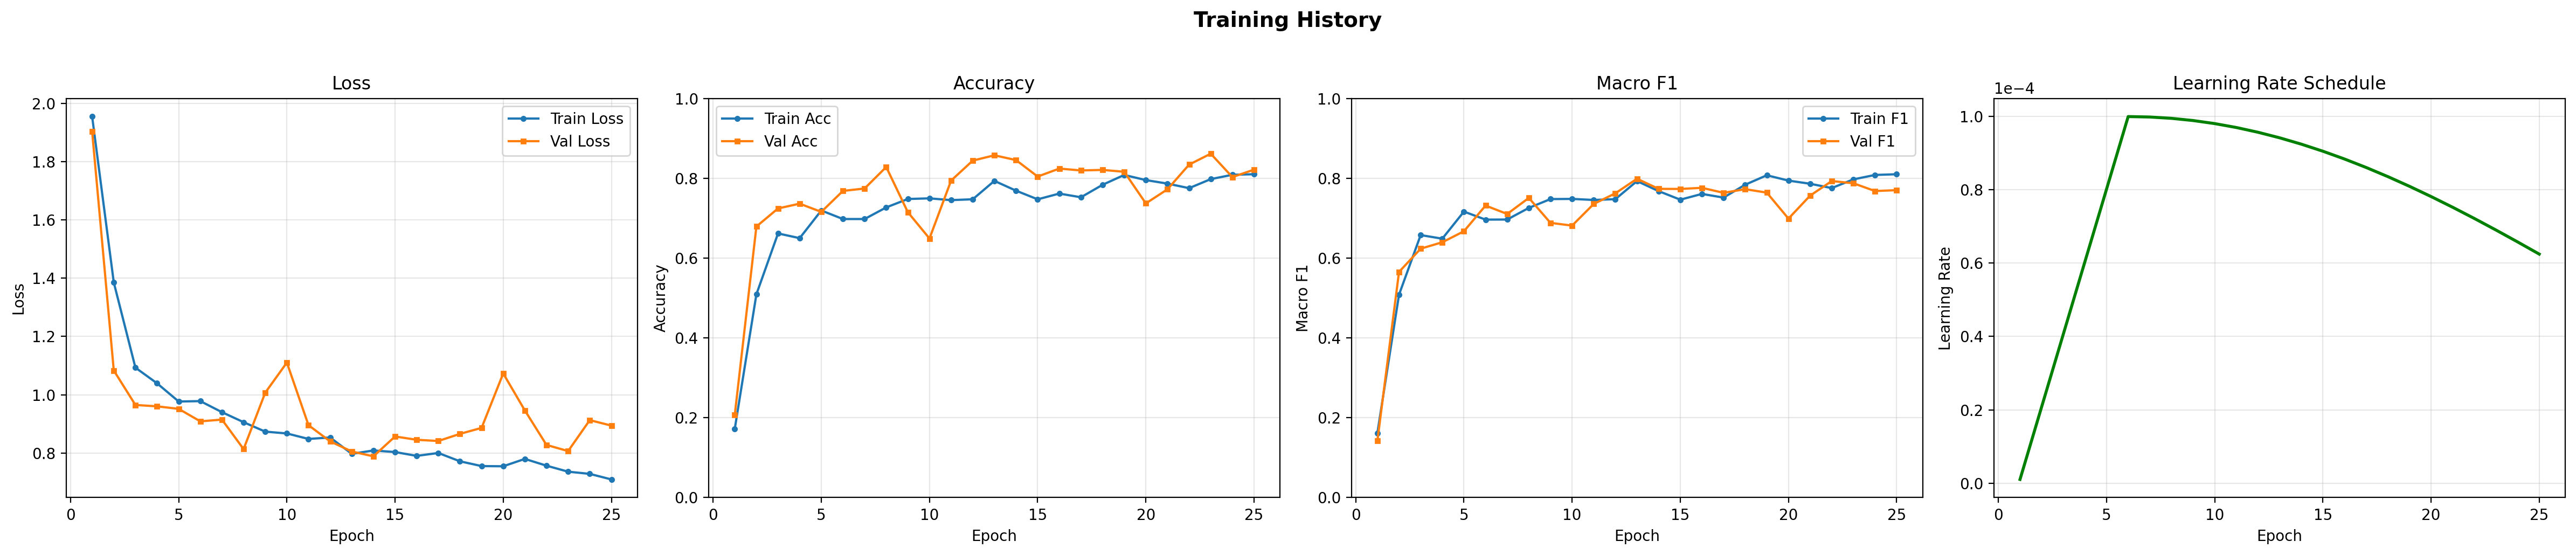
\includegraphics[width=1.15\textwidth]{figures/swin_training_history.png}}
    \caption{Swin-Tiny}
\end{subfigure}
\caption[]{Training history for all four models (continued).}
\end{figure}

Notable differences in convergence behavior include:
\begin{itemize}
    \item \textbf{EfficientNet-B0 and ResNet50} both achieved their best validation performance at epoch 39, with 11 subsequent epochs showing no improvement.
    \item \textbf{DenseNet121} reached its best performance at epoch 49 out of 50, suggesting that the dense connectivity pattern requires more training iterations to fully converge.
    \item \textbf{Swin-Tiny} triggered early stopping at epoch 25 (best at epoch 13), indicating faster convergence but also a tendency to overfit earlier than the CNN models on this relatively small dataset.
\end{itemize}

\subsection{Confusion Matrices}

Figure~\ref{fig:confusion_matrices} presents the normalized confusion matrices for all four models. The most common misclassification pattern across all models is the confusion between MEL and NV, which is clinically expected given their morphological similarity. BKL is also frequently confused with NV.

\begin{figure}[H]
\centering
\begin{subfigure}{\textwidth}
    \makebox[\textwidth][c]{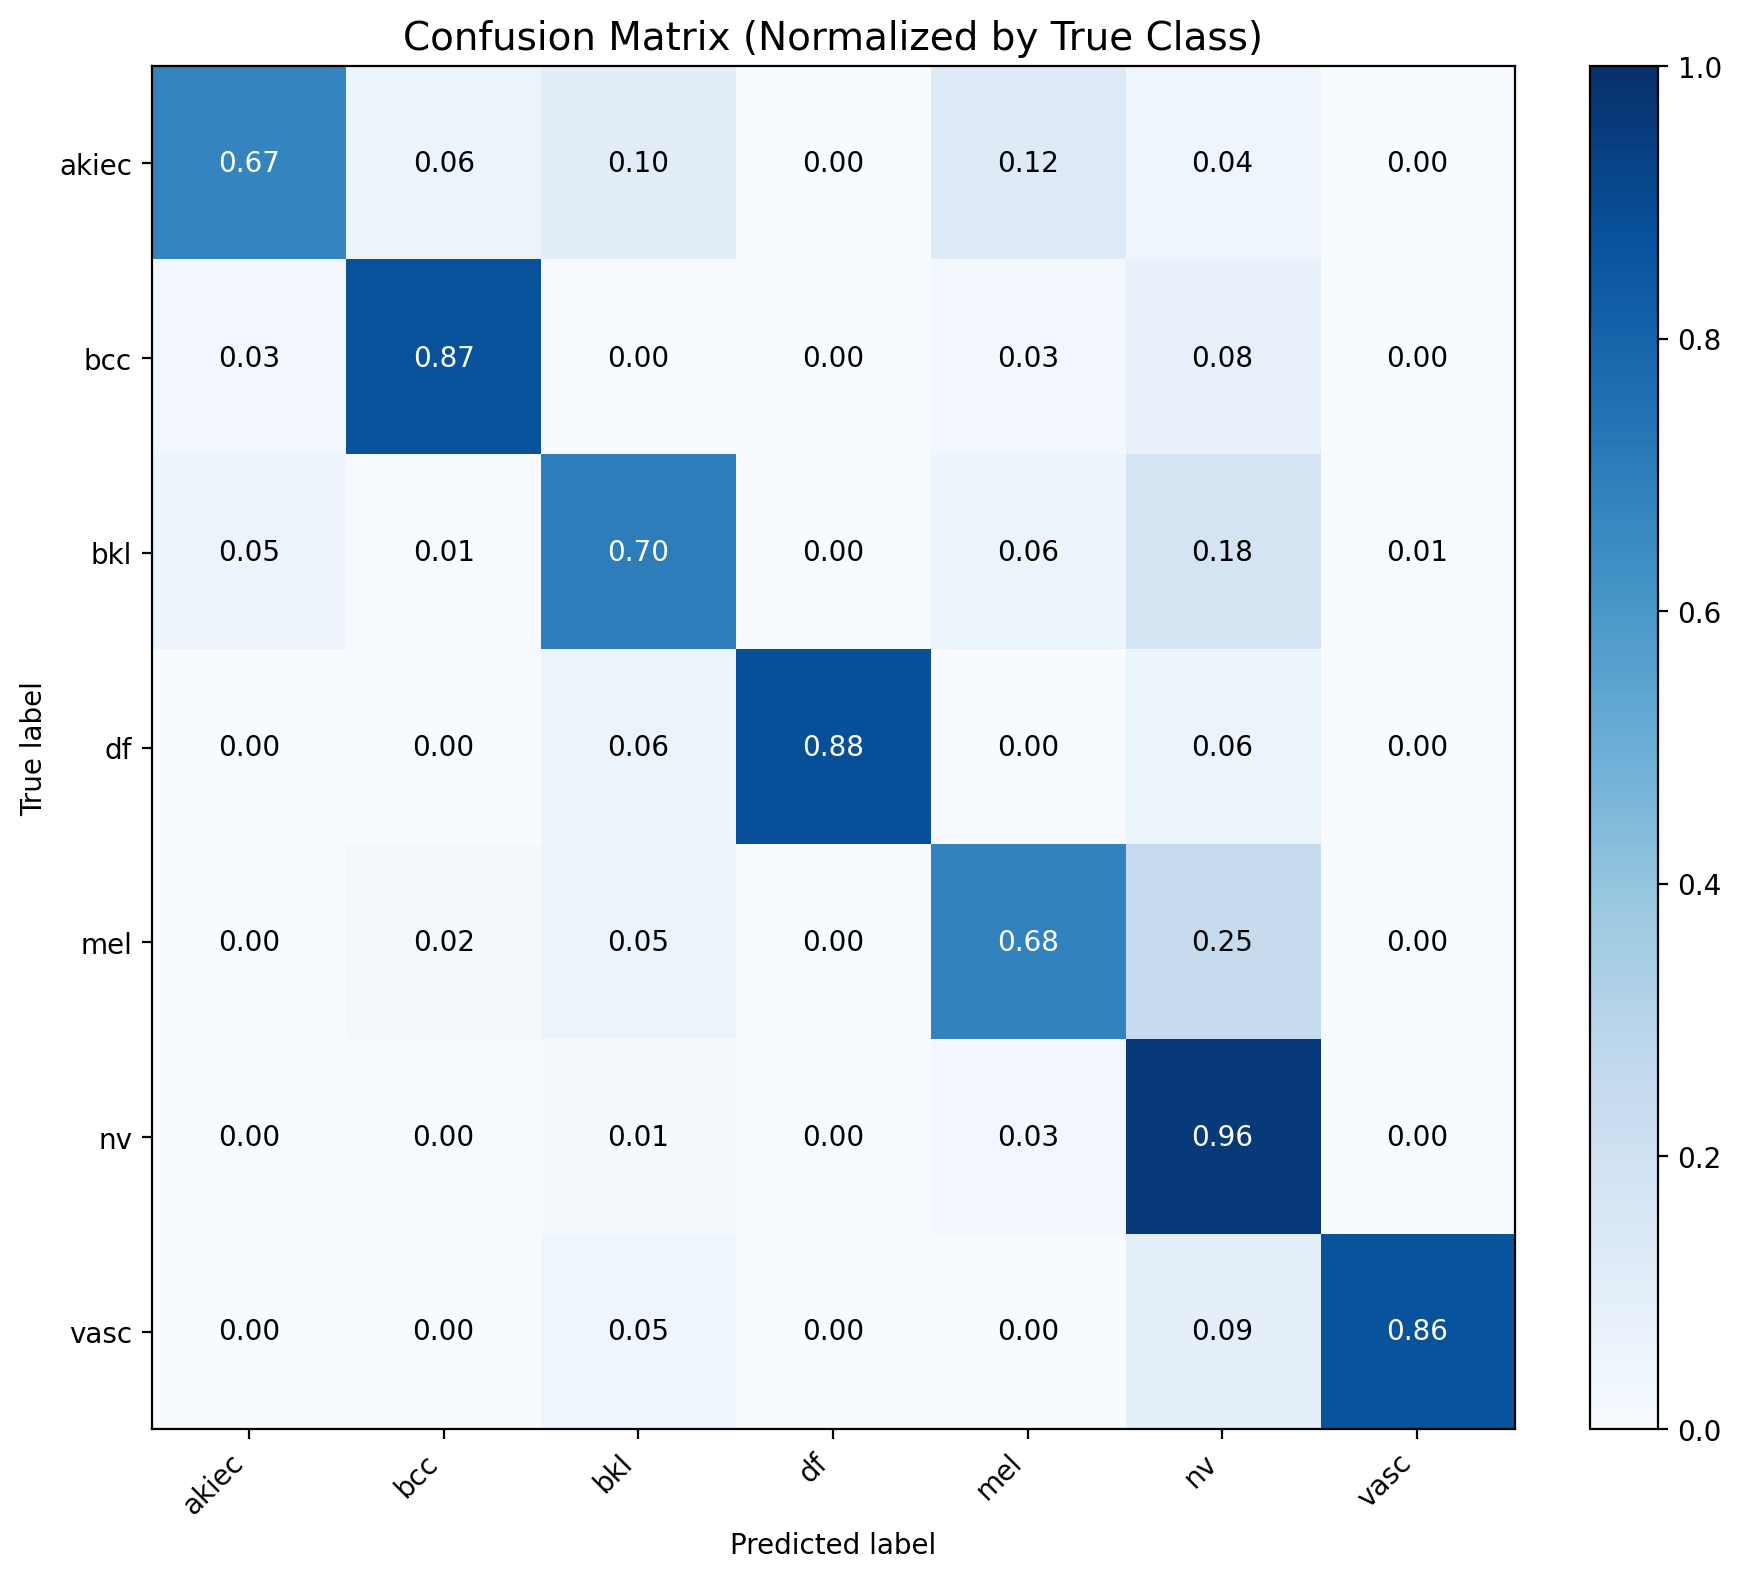
\includegraphics[width=0.9\textwidth]{figures/eb0_confusion_matrix.png}}
    \caption{EfficientNet-B0}
\end{subfigure}

\vspace{0.6cm}

\begin{subfigure}{\textwidth}
    \makebox[\textwidth][c]{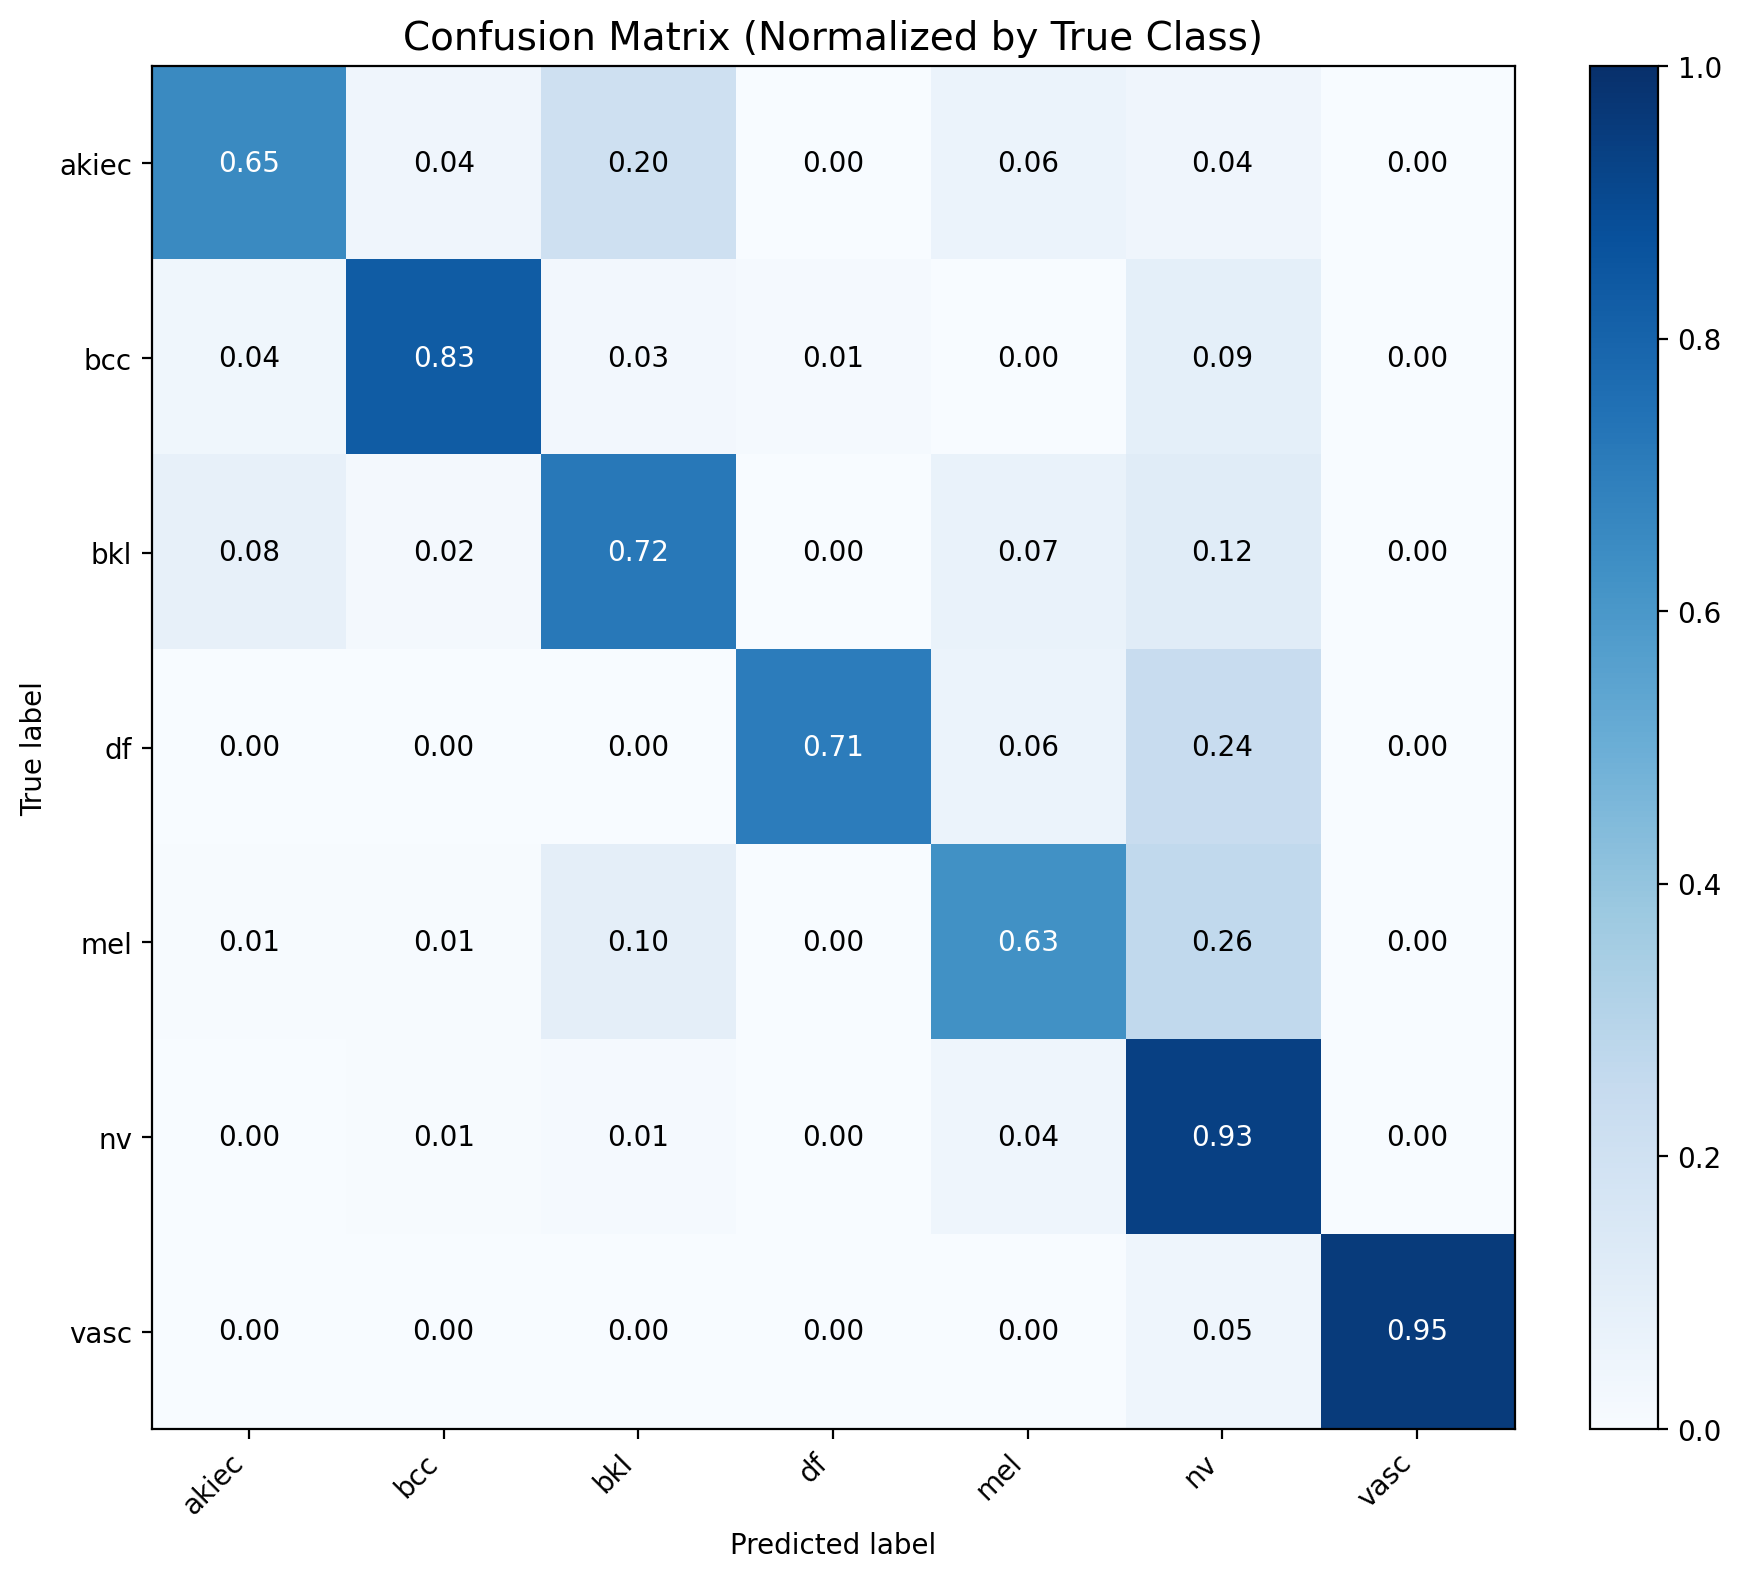
\includegraphics[width=0.9\textwidth]{figures/rn50_confusion_matrix.png}}
    \caption{ResNet50}
\end{subfigure}
\caption{Normalized confusion matrices for all four models on the test set.}
\label{fig:confusion_matrices}
\end{figure}

\begin{figure}[H]
\ContinuedFloat
\centering
\begin{subfigure}{\textwidth}
    \makebox[\textwidth][c]{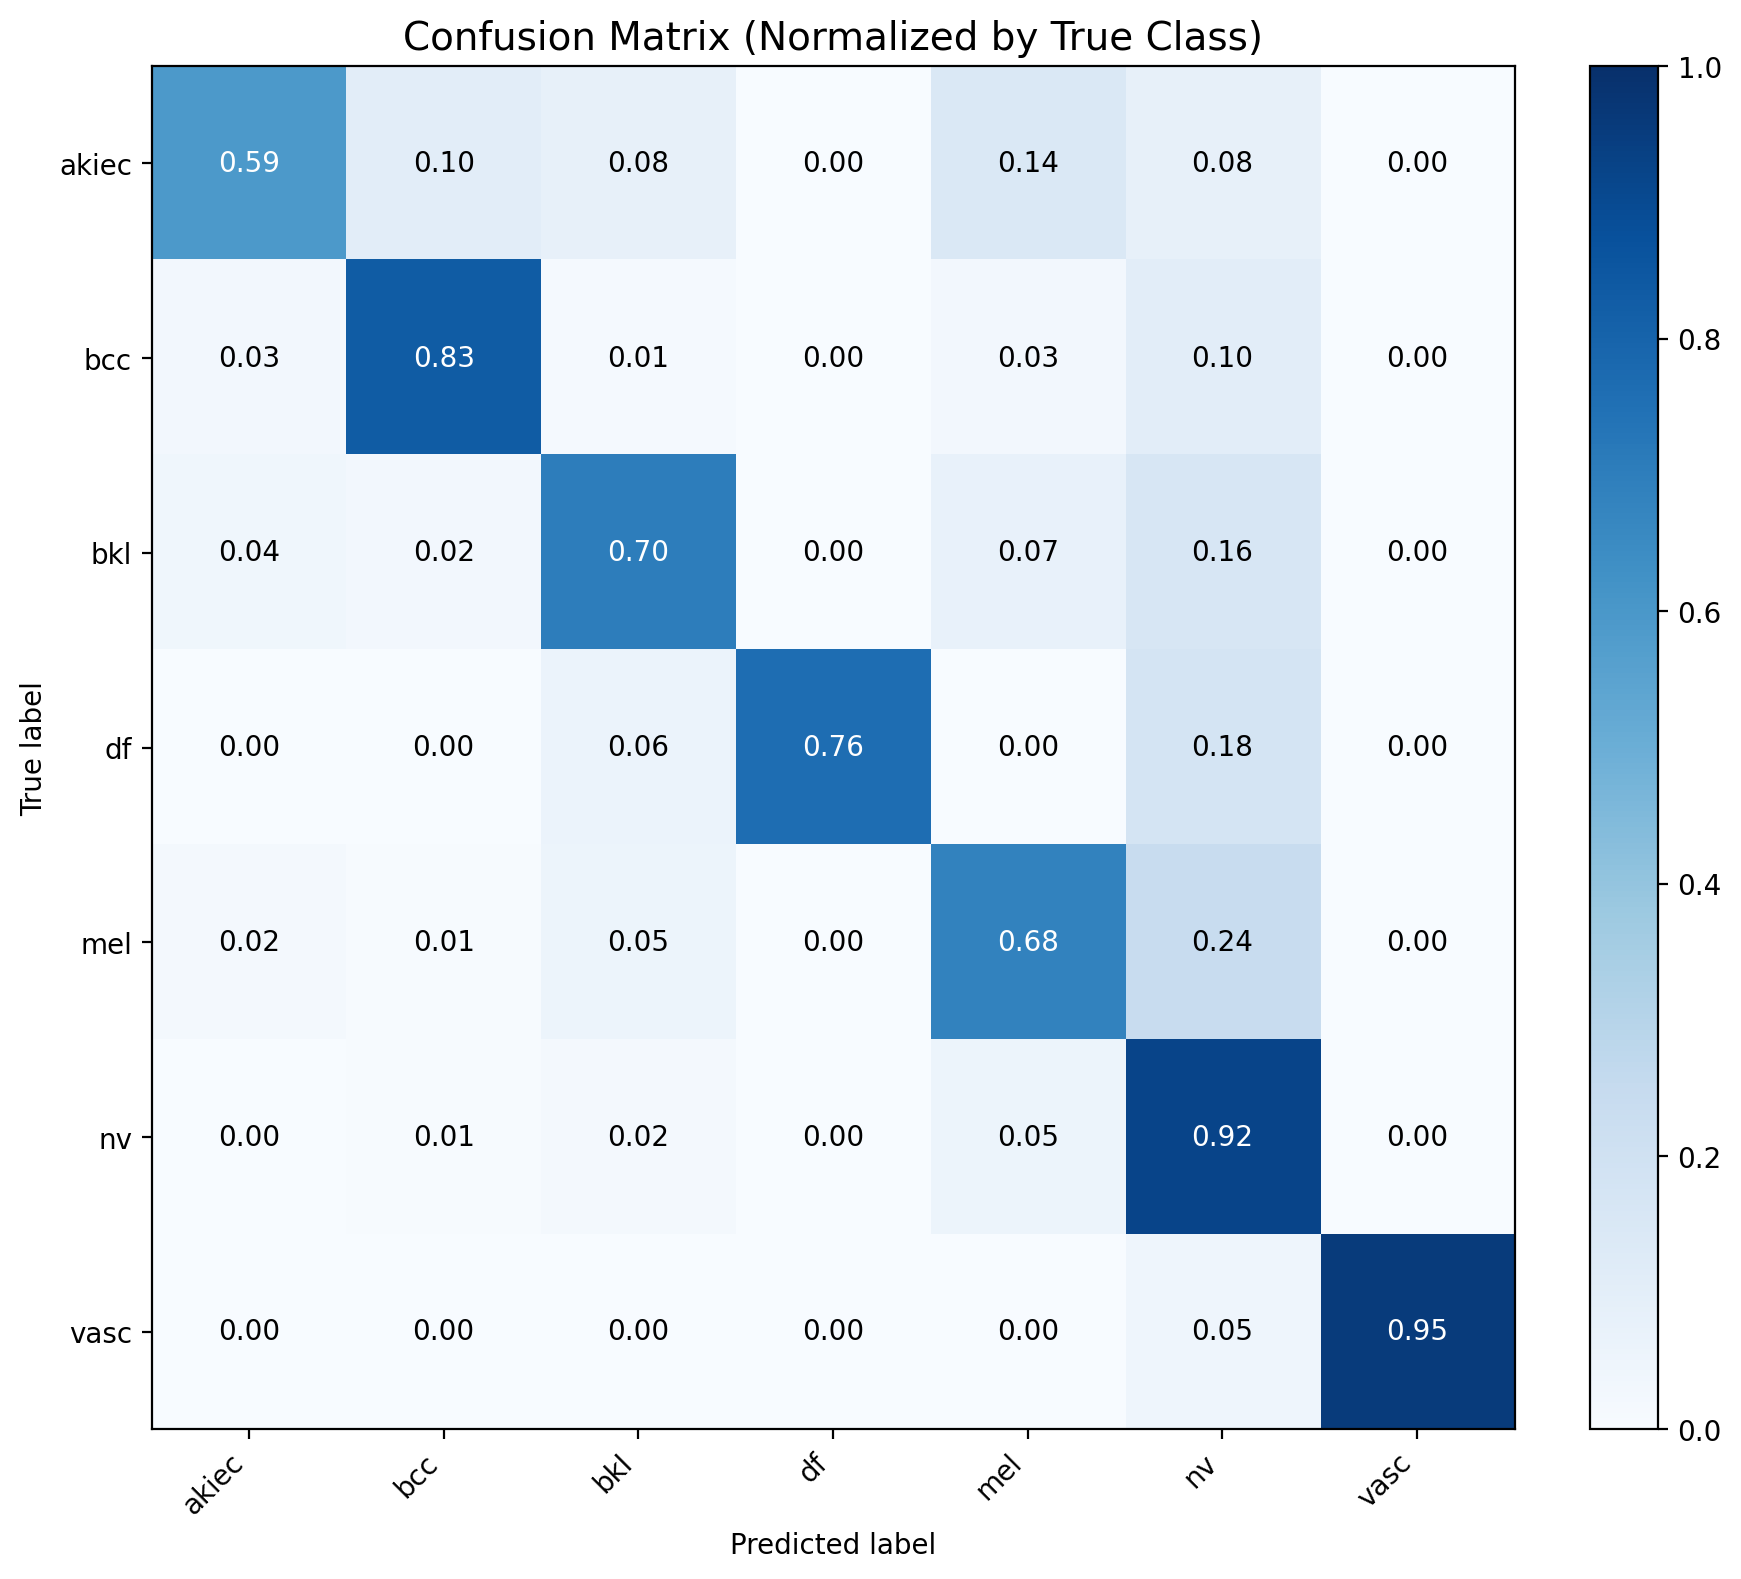
\includegraphics[width=0.9\textwidth]{figures/dn121_confusion_matrix.png}}
    \caption{DenseNet121}
\end{subfigure}

\vspace{0.6cm}

\begin{subfigure}{\textwidth}
    \makebox[\textwidth][c]{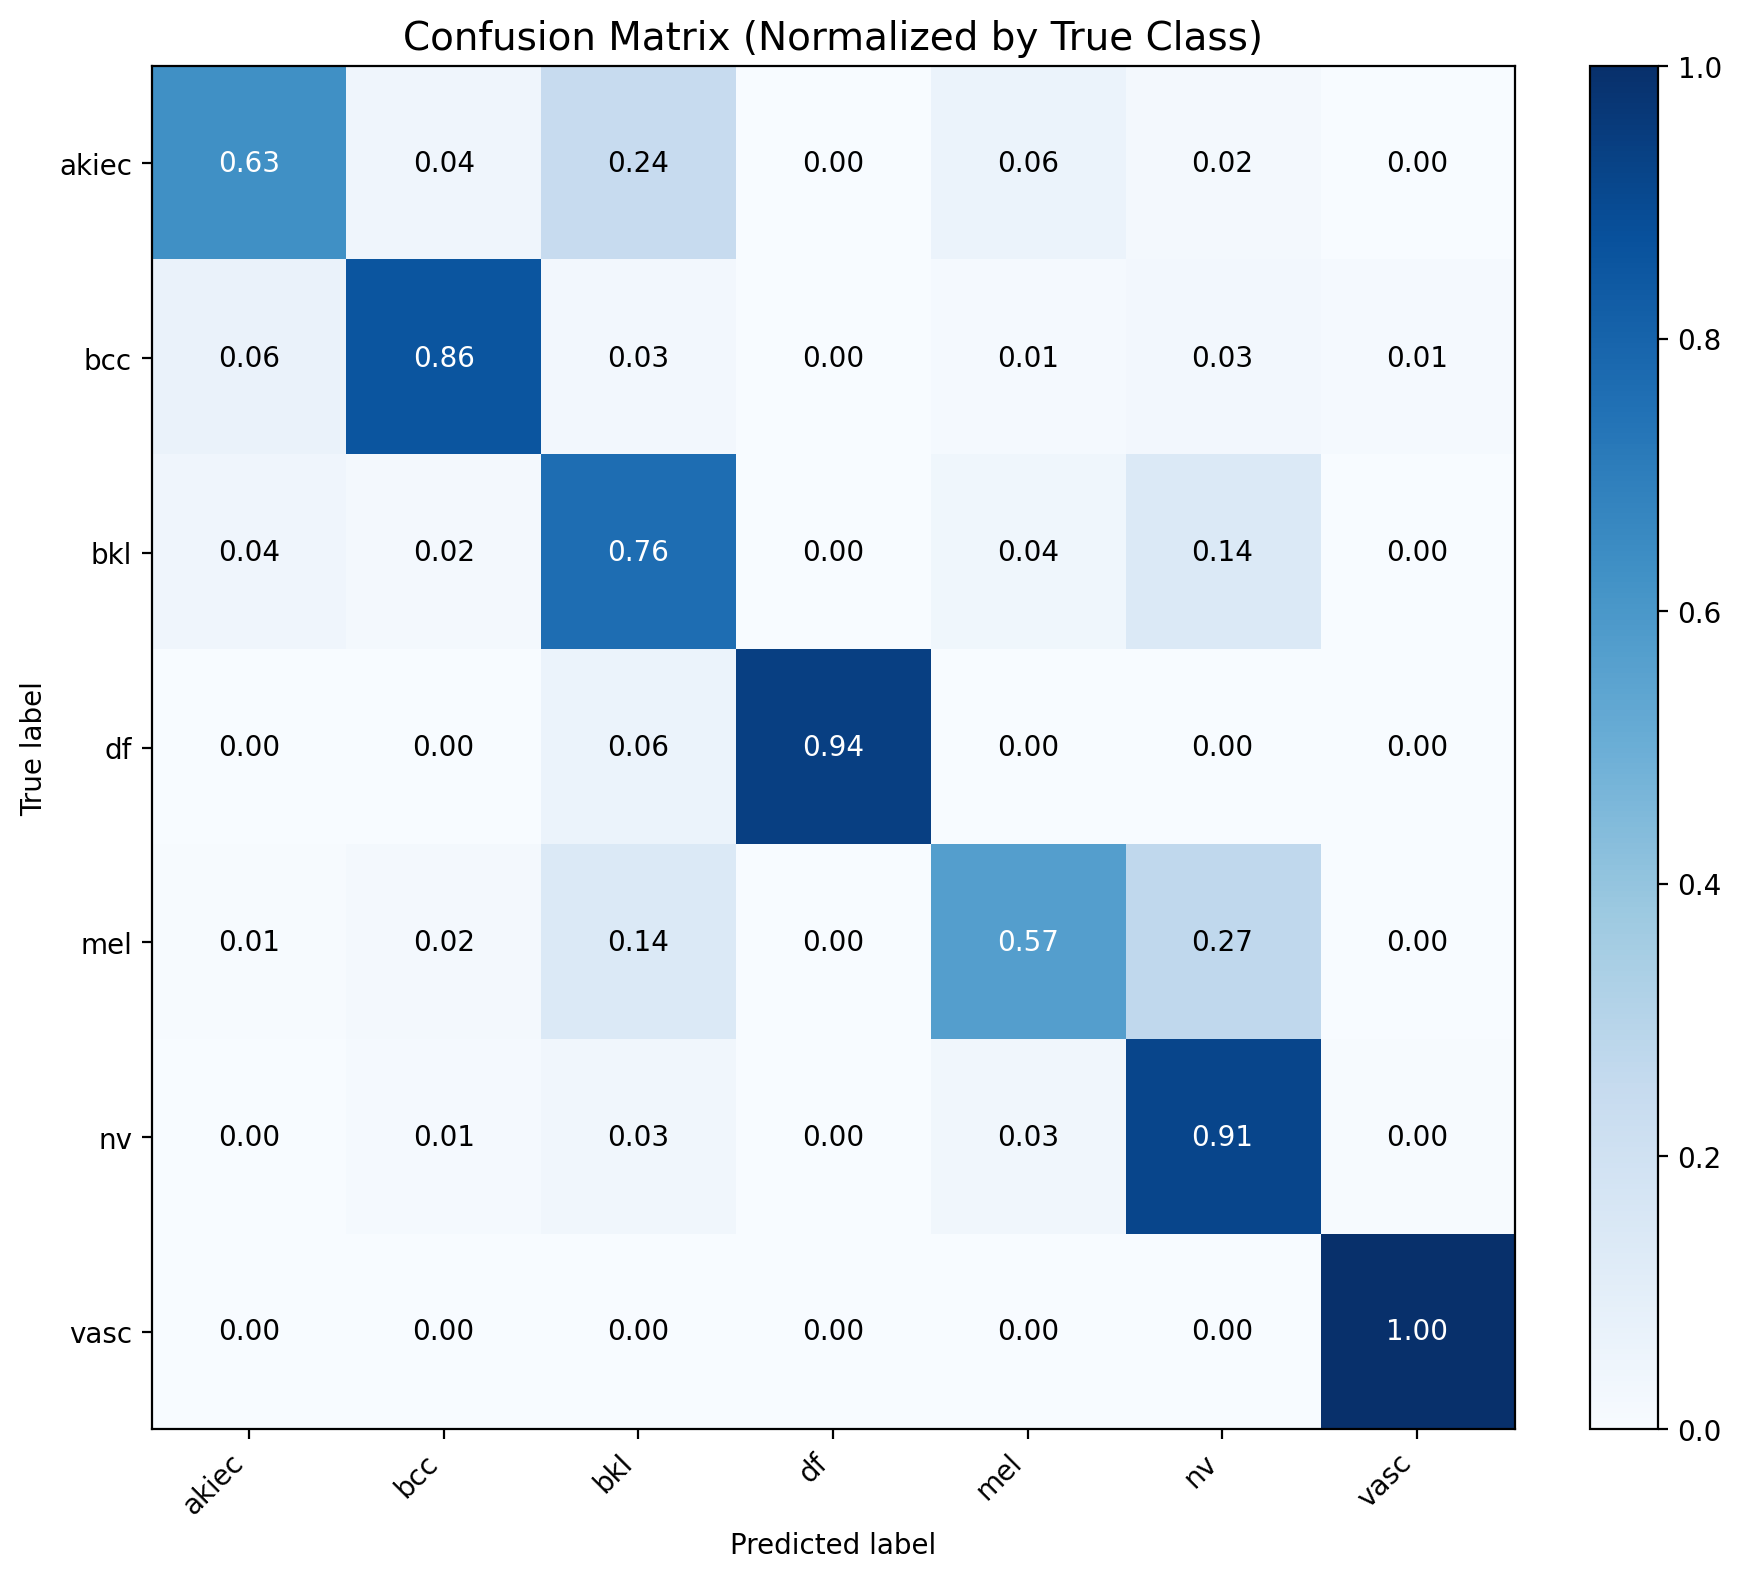
\includegraphics[width=0.9\textwidth]{figures/swin_confusion_matrix.png}}
    \caption{Swin-Tiny}
\end{subfigure}
\caption[]{Normalized confusion matrices for all four models on the test set (continued).}
    \end{figure}


    \section{Ensemble Results}

A soft-voting ensemble~\cite{ganaie2022ensemble} combining all four models achieved the best overall performance, as shown in Table~\ref{tab:ensemble_results}.

\begin{table}[H]
\centering
\caption{Comparison of individual models versus the ensemble on the test set.}
\label{tab:ensemble_results}
\begin{tabular}{lccccc}
\toprule
\textbf{Model} & \textbf{Accuracy} & \textbf{Macro F1} & \textbf{AUC} & \textbf{MCC} & \textbf{Kappa} \\
\midrule
EfficientNet-B0  & 0.8836 & 0.8311 & 0.9522 & 0.7721 & 0.7710 \\
ResNet50         & 0.8603 & 0.7902 & 0.9565 & 0.7310 & 0.7309 \\
DenseNet121      & 0.8543 & 0.7967 & 0.9587 & 0.7209 & 0.7206 \\
Swin-Tiny        & 0.8490 & 0.7855 & 0.9600 & 0.7157 & 0.7150 \\
\midrule
\textbf{Ensemble (4 models)} & \textbf{0.8949} & \textbf{0.8446} & \textbf{0.9802} & \textbf{0.7956} & \textbf{0.7949} \\
\bottomrule
\end{tabular}
\end{table}

The ensemble improved accuracy by +1.13\% over the best individual model (EfficientNet-B0) and, more importantly, boosted the macro AUC from 0.952 to \textbf{0.980}---a substantial improvement indicating near-perfect probability calibration across all classes. The melanoma F1-score improved from 0.695 to 0.744 (+4.9\%), demonstrating that architectural diversity helps reduce class-specific errors.

\begin{figure}[H]
\centering
\begin{subfigure}{0.46\textwidth}
    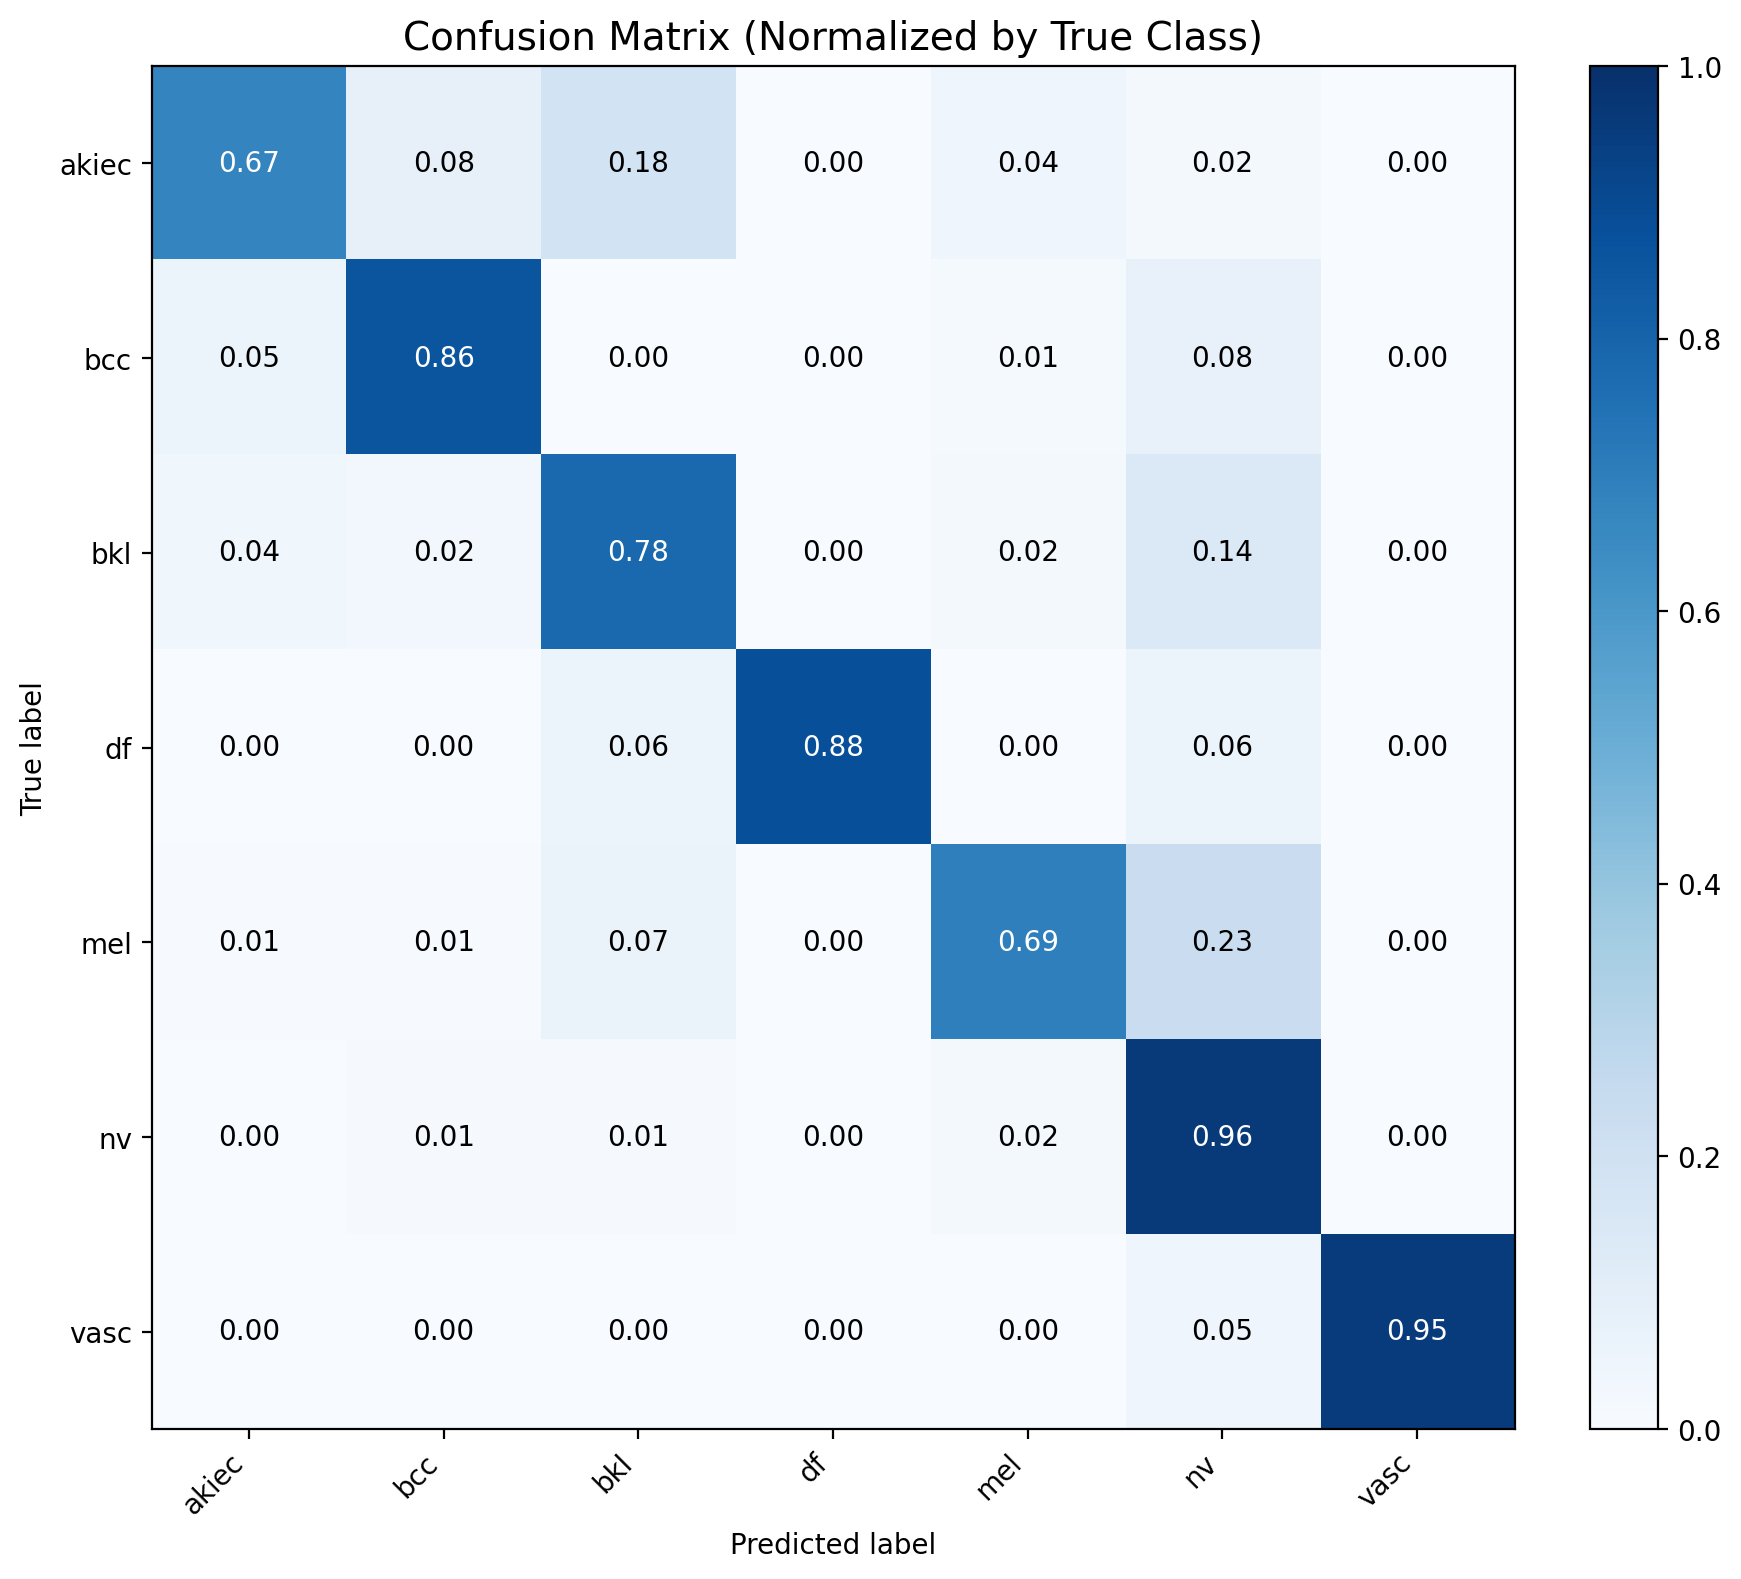
\includegraphics[width=\textwidth]{figures/ensemble_confusion_matrix.png}
    \caption{Confusion matrix}
\end{subfigure}
\hfill
\begin{subfigure}{0.46\textwidth}
    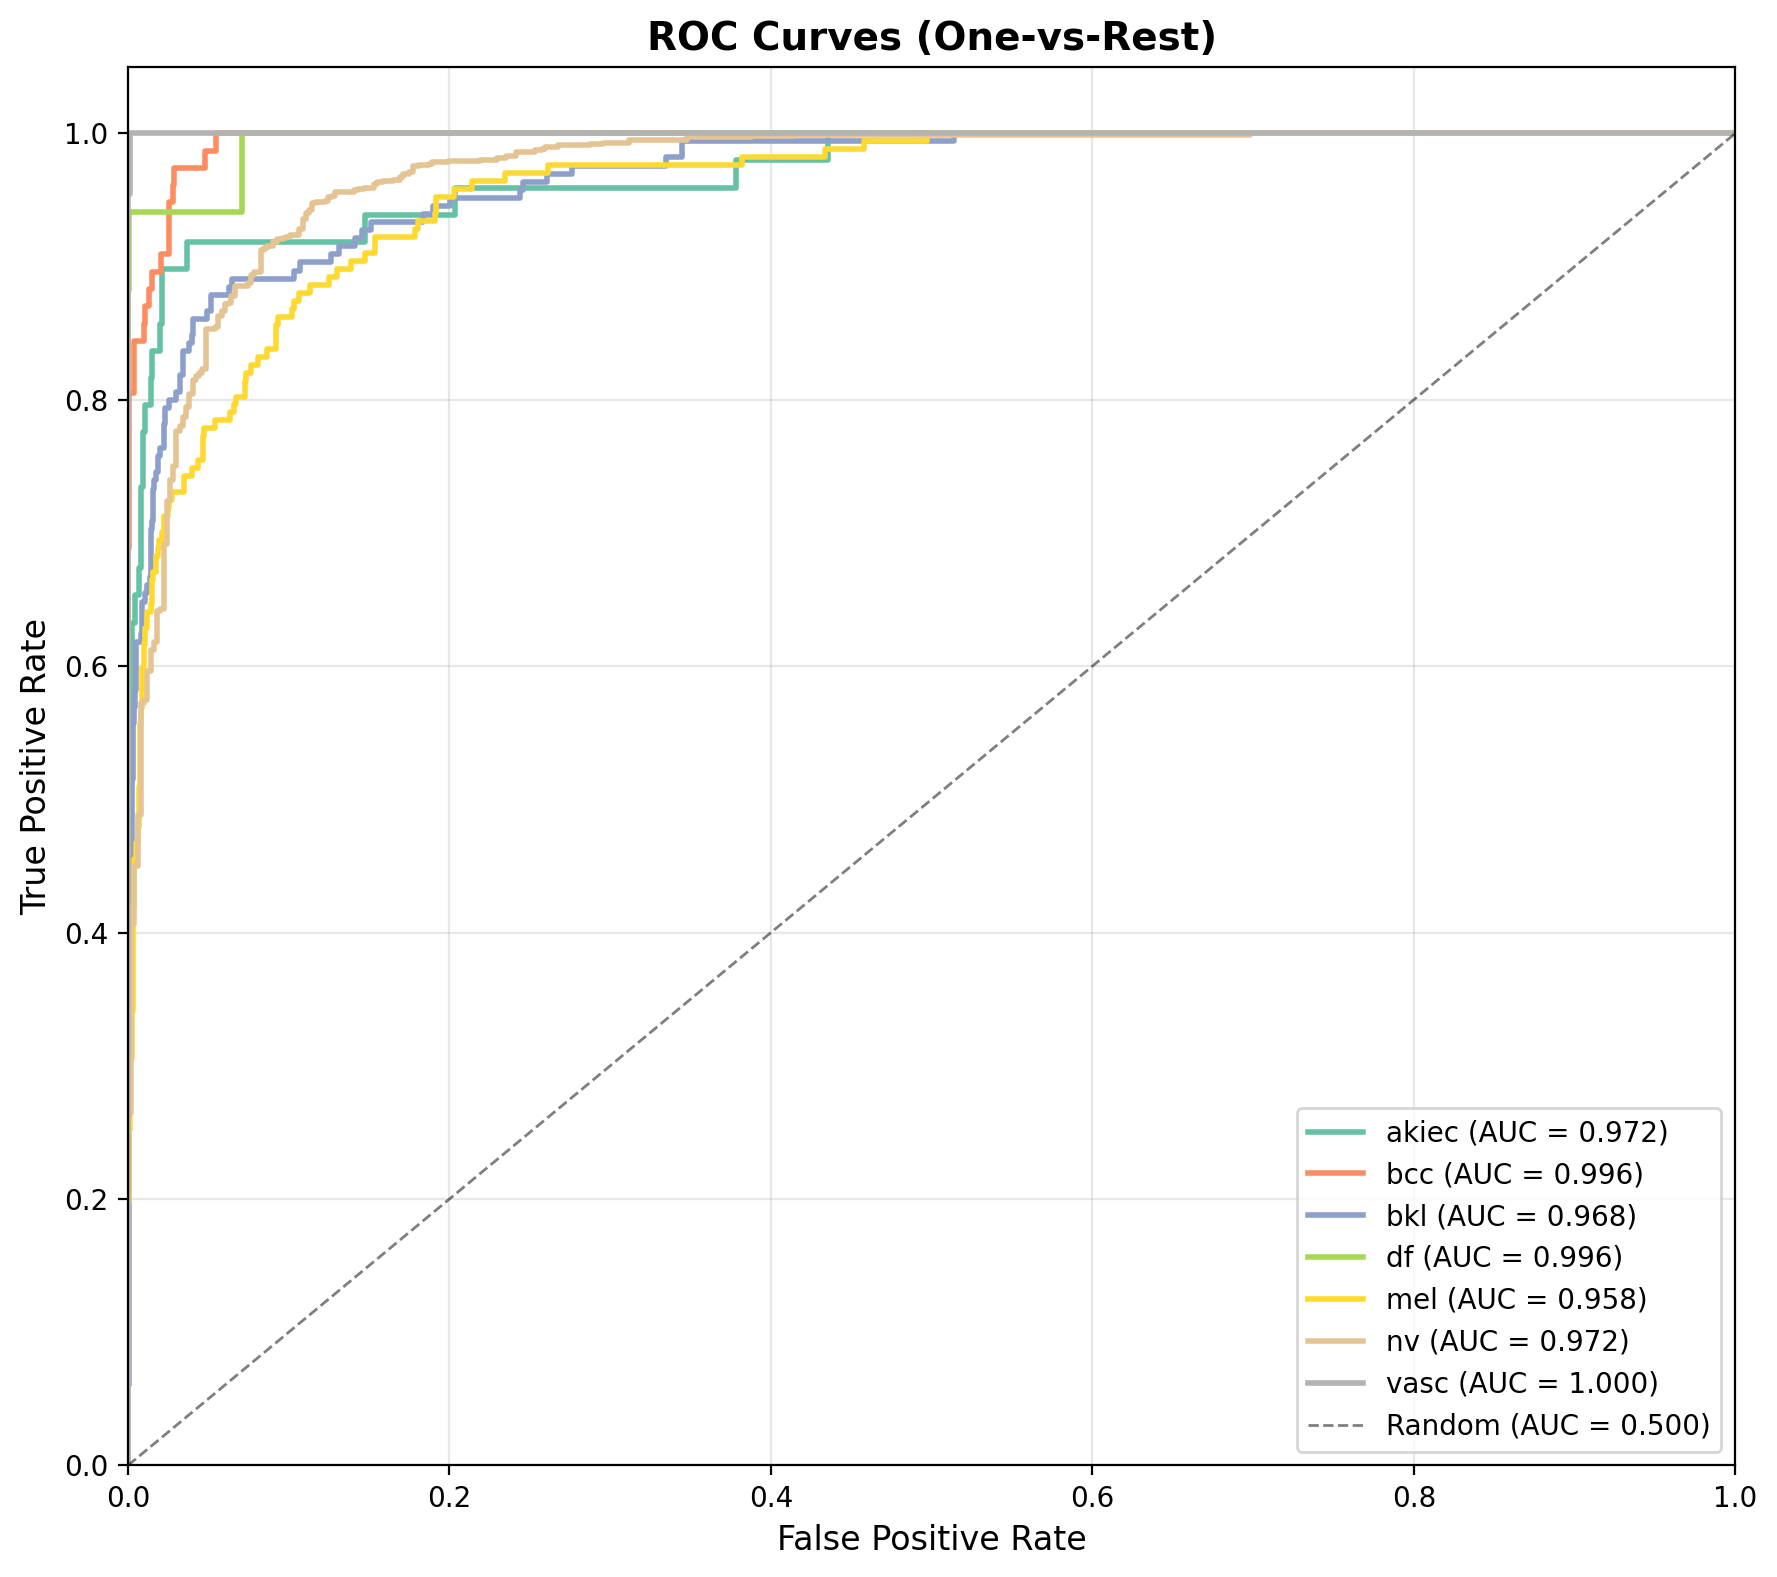
\includegraphics[width=\textwidth]{figures/ensemble_roc_curves.png}
    \caption{ROC curves}
\end{subfigure}
\caption{Ensemble model performance: (a) normalized confusion matrix and (b) per-class ROC curves with AUC values.}
\label{fig:ensemble_results}
\end{figure}

Table~\ref{tab:ensemble_per_class} shows the per-class ensemble performance compared to the best individual model.

\begin{table}[H]
\centering
\caption{Per-class performance of the ensemble versus the best individual model (EfficientNet-B0).}
\label{tab:ensemble_per_class}
\begin{tabular}{lcccccc}
\toprule
\textbf{Class} & \textbf{EB0 F1} & \textbf{Ens. F1} & \textbf{$\Delta$F1} & \textbf{EB0 AUC} & \textbf{Ens. AUC} & \textbf{$\Delta$AUC}\\
\midrule
AKIEC & 0.717 & 0.710 & $-$0.007 & 0.921 & 0.972 & +0.051 \\
BCC   & 0.865 & 0.825 & $-$0.040 & 0.984 & 0.996 & +0.012 \\
BKL   & 0.758 & 0.796 & +0.038  & 0.938 & 0.968 & +0.030 \\
DF    & 0.938 & 0.938 &  0.000  & 0.963 & 0.996 & +0.033 \\
MEL   & 0.695 & 0.744 & +0.049  & 0.913 & 0.958 & +0.045 \\
NV    & 0.940 & 0.946 & +0.006  & 0.946 & 0.972 & +0.026 \\
VASC  & 0.905 & 0.955 & +0.050  & 1.000 & 1.000 &  0.000 \\
\bottomrule
\end{tabular}
\end{table}

\section{Grad-CAM Interpretability Analysis}

To verify that the models are making predictions based on clinically relevant features, Grad-CAM heatmaps were generated for all four models on test-set samples. Figure~\ref{fig:gradcam_grid} shows a comprehensive comparison across all seven disease classes.

\begin{figure}[H]
\centering
\includegraphics[width=\textwidth]{figures/gradcam_class_grid.png}
\caption{Grad-CAM heatmap comparison across all seven classes and four models. Red regions indicate high model attention; blue regions indicate low attention. Green titles indicate correct predictions; red titles indicate misclassifications.}
\label{fig:gradcam_grid}
\end{figure}

Key observations from the Grad-CAM analysis:

\begin{itemize}
    \item \textbf{All models consistently focus on the lesion region} rather than surrounding healthy skin, background artifacts, or ruler markings. This confirms that the learned representations are clinically relevant.
    \item \textbf{EfficientNet-B0 produces the most focused heatmaps}, concentrating attention tightly on the lesion boundary---a feature that dermatologists also prioritize when assessing border irregularity.
    \item \textbf{Swin-Tiny exhibits broader attention patterns}, consistent with the global receptive field of self-attention. While this captures the overall shape of the lesion, it may include some non-discriminative surrounding tissue.
    \item \textbf{For melanoma samples} (Figure~\ref{fig:gradcam_mel}), all models attend to areas of asymmetric pigmentation and irregular borders, which align with the ABCDE criteria used in clinical dermatology (Asymmetry, Border irregularity, Color variation, Diameter, Evolution).
\end{itemize}

\begin{figure}[H]
\centering
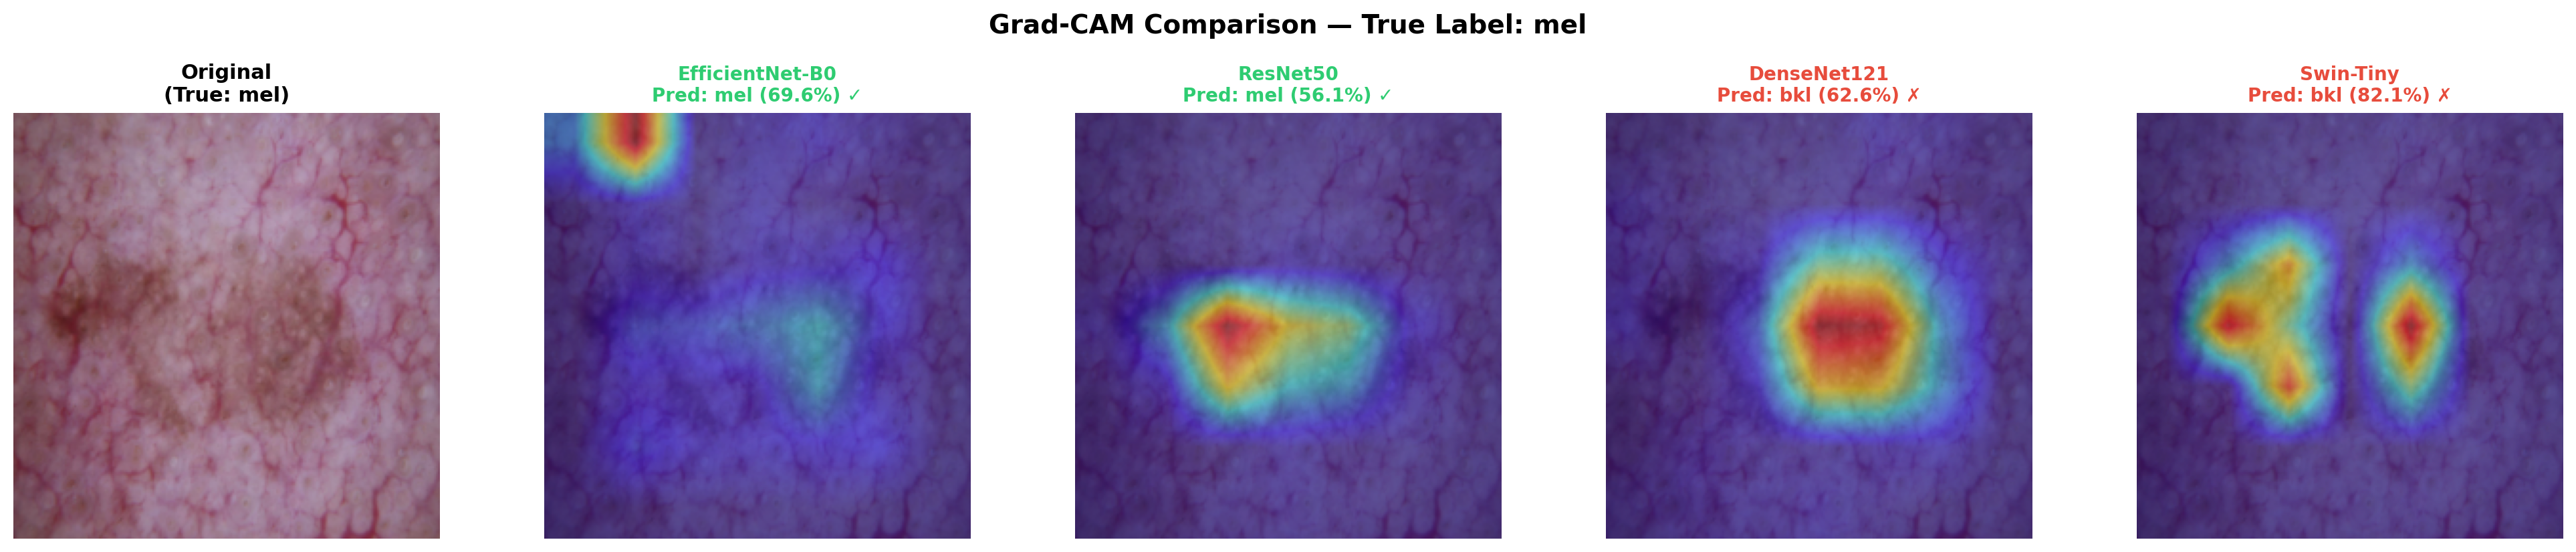
\includegraphics[width=\figwidth]{figures/gradcam_mel_sample.png}
\caption{Grad-CAM visualization for a melanoma sample. All four models correctly focus on the irregularly pigmented lesion area.}
\label{fig:gradcam_mel}
\end{figure}

\section{Ablation Study}

To quantify the contribution of each component in our training pipeline, an ablation study was conducted using EfficientNet-B0 as the base model. In each experiment, a single component was removed while keeping all others fixed.

\begin{table}[H]
\centering
\caption{Ablation study results on EfficientNet-B0. Each row shows the effect of removing one component from the full pipeline. $\Delta$ indicates the change relative to the full model.}
\label{tab:ablation}
\begin{tabular}{lccccc}
\toprule
\textbf{Configuration} & \textbf{Accuracy} & \textbf{Macro F1} & \textbf{AUC} & \textbf{Kappa} & \textbf{$\Delta$ Macro F1}\\
\midrule
Full Pipeline (baseline) & \textbf{0.8836} & \textbf{0.8311} & 0.9522 & \textbf{0.7710} & --- \\
\midrule
$-$ Mixup / CutMix       & 0.8589 & 0.7860 & 0.9486 & 0.7383 & $-$0.0451 \\
$-$ Weighted Sampler     & 0.8762 & 0.8041 & 0.9521 & 0.7487 & $-$0.0270 \\
$-$ Label Smoothing      & 0.8776 & 0.8000 & 0.9674 & 0.7568 & $-$0.0311 \\
$-$ Advanced Augmentation& 0.8896 & 0.8204 & \textbf{0.9664} & 0.7772 & $-$0.0107 \\
\bottomrule
\end{tabular}
\end{table}

The ablation results presented in Table~\ref{tab:ablation} provide strong empirical justification for the proposed training pipeline. The key findings are:

\textbf{Mixup and CutMix are the most critical components.} Removing these spatial and label-mixing regularizations~\cite{zhang2018mixup,yun2019cutmix} resulted in the most severe performance degradation, causing a massive drop of 4.5\% in Macro F1. Without the synthetic examples generated by Mixup and CutMix, the model quickly memorized the rare classes during training and failed to generalize to the test set, leading to early overfitting.

\textbf{Label Smoothing prevents overconfidence.} Removing Label Smoothing~\cite{szegedy2016rethinking,muller2019does} caused a 3.1\% drop in Macro F1. Interestingly, removing label smoothing \textit{increased} the AUC from 0.952 to 0.967, suggesting that while label smoothing improves hard classification decisions by preventing overconfident predictions, it slightly reduces the sharpness of the probability ranking. In skin lesion classification, borders between classes like Melanoma and Nevi are highly ambiguous. Label smoothing acts as a soft margin, preventing the model from becoming overly confident in ambiguous predictions and improving the separation of classes.

\textbf{Weighted Random Sampler is essential for minority classes.} Removing the weighted sampler~\cite{buda2018systematic} led to a 2.7\% drop in Macro F1. Without it, the model prioritized the heavily dominant Nevi class (which accounts for over 60\% of the dataset) at the expense of rare but critical classes like Dermatofibroma and Vascular Lesions.

\textbf{Advanced Augmentations slightly hurt Accuracy but improve F1.} Interestingly, removing advanced augmentations~\cite{shorten2019survey} (such as RandomResizedCrop, Gaussian Blur, and Random Erasing~\cite{zhong2020random}) actually increased raw Accuracy to 88.96\% but decreased the Macro F1 score by 1.07\%. This highlights the tradeoff in imbalanced datasets: aggressive augmentation makes the training task harder, slightly reducing the accuracy on the easy majority class, but significantly improves the model's robustness on the harder, less-represented classes.
